% ----- formatovani dokumentu -----------------------------------------------
\documentclass[12pt,a4paper,titlepage,final]{report}
\usepackage[utf8]{inputenc}
\usepackage[T1, IL2]{fontenc}
\usepackage{graphicx}
\usepackage{epstopdf}
\usepackage[margin=2cm]{caption}
\usepackage[top=3cm, left=2cm, right=2cm, text={17cm, 24cm}, ignorefoot]{geometry}
\usepackage{color}
\usepackage{url}
\usepackage{setspace}
\singlespacing
\usepackage[square, numbers]{natbib} 
\usepackage{float}
\pagestyle{plain}
\pagenumbering{arabic}
\setcounter{page}{1}
\setcounter{secnumdepth}{-1}
\setlength{\parindent}{1cm}	
\usepackage{natbib}
\usepackage{amsmath}
\usepackage{tocloft}
\usepackage{esvect}
\usepackage{amssymb}
\usepackage{gensymb}
\usepackage{subcaption}
\usepackage[algoruled,boxed,lined,longend]{algorithm2e}
\usepackage{mathtools}

\DeclareMathOperator{\dis}{d}

  \newenvironment{czechalgorithm}[1][htb]
  {\renewcommand{\algorithmcfname}{Algoritmus}% Update algorithm name
   \begin{algorithm}[#1]%
  }{\end{algorithm}}

% ----- vyberte jazyk -------------------------------------------------------
\usepackage[english,czech]{babel}
%\usepackage[english]{babel}

% ----- dopiste titulky -----------------------------------------------------
\newcommand\Course{Grafické a multimediální procesory}
\newcommand\WorkTitle{Aplikace simulace vody pomocí celulárních automatů na GPU}
\newcommand\AuthorA{Petr Flajšingr}
\newcommand\AuthorAEmail{xflajs00@stud.fit.vutbr.cz}
\newcommand\AuthorB{Igor Frank}
\newcommand\AuthorBEmail{xfrank12@stud.fit.vutbr.cz}
\newcommand\Faculty{Fakulta Informačních Technologií}
\newcommand\School{Vysoké Učení Technické v Brně}

\usepackage[
pdftitle={\WorkTitle},
pdfauthor={\AuthorA}
bookmarks=true,
colorlinks=true,
breaklinks=true,
urlcolor=blue,
citecolor=blue,
linkcolor=blue,
unicode=true,
]
{hyperref}


% ----- titulni strana ------------------------------------------------------

\begin{document}
	\begin{titlepage}
	\begin{center}
		
\includegraphics[height=5cm]{images/logo.eps}
	\end{center}
	\vfill
	\begin{center}
		\begin{Large}
			\Course\\
		\end{Large}
		\bigskip
		\begin{Huge}
			\WorkTitle\\
		\end{Huge}
	\end{center}
	\vfill
	\begin{center}
		\begin{large}
			\today
		\end{large}
	\end{center}
	\vfill
	\begin{flushleft}
		\begin{large}
			\begin{tabular}{lll}
				Autoři: & \AuthorA, & \url{\AuthorAEmail} \\
				& \AuthorB, & \url{\AuthorBEmail} \\
				& \Faculty \\
				& \School \\
			\end{tabular}
		\end{large}
	\end{flushleft}
\end{titlepage}		

\section{Úvod}
Tato práce se zabývá návrhem a implementací algoritmů pro simulaci vody pomocí celulárních automatů na GPU s využitím jazyka C++ a knihovny OpenGL. První implementovaná metoda spadá do kategorie typických celulárních automatů. Druhá metoda se snaží být fyzikálně přesnější s využitím směrového vektoru pro určení směru pohybu vody.


\section{Implementace}
V obou metodách využíváme dvou bufferů -- jeden pro čtení hodnot, které jsou dostupné z minulého kroku (případně inicializace) simulace. Druhý buffer slouží k zápisu nových hodnot. Po každém kroku simulace jsou tyto buffery prohozeny. Obě metody jsou implementovány za pomocí compute shaderů\footnote{\url{https://www.khronos.org/opengl/wiki/Compute_Shader}}.

Obě metody používají Von Neumannovo sousedství. Simulace podporují čtyři typy buněk:
\begin{itemize}
    \item Solid -- reprezentuje buňku, která nemůže obsahovat kapalinu.
    \item Fluid -- buňka, která může obsahovat kapalinu.
    \item Sink -- buňka, která maže veškerou kapalinu, která do ní přiteče.
    \item Source -- buňka, která vždy obsahuje maximální množství kapaliny.
\end{itemize}

\subsection{První metoda}
Jedná se o dvou-průchodovou metodu, kdy v prvním průchodu vypočteme změnu obsahu tekutiny ve vertikálním směru. V tomto průchodu se snažíme co nejvíce kapaliny přesunout z aktuální buňky do buňky o jedno níže. Pomocí prvního průchodu tak jednoduše simulujeme gravitaci. V druhém průchodu se pokoušíme veškerou kapalinu která se již nedokázala vměstnat do spodní buňky rovnoměrně přesunout do buňek okolních. Jako okolí jsme si zvolili jednoduché Von Neumanovo 4-okolí. Celý algoritmus je následující:
\begin{enumerate}
    \item Vypočítej množství přítoku podle rovnice \ref{eq:cell_vert}.
    \item Vypočítej množství odtoku podle rovnice \ref{eq:cell_vert}.
    \item Omez hodnoty podle množství tekutiny v současné buňce a podle volného místa v buňce spodní.
    \item Ulož změnu do zapisovacího bufferu.
    \item Spočítej kolik sousedních buněk má nižší hladinu tekutiny.
    \item Pro všechny horizontální sousední buňky proveď následující:
    \item Vypočítej přítok ze sousední buňky podle rovnice \ref{eq:cell_hori}.
    \item Vypočítej odtok do sousední buňky podle rovnice \ref{eq:cell_hori}.
    \item Přepočítej obsah aktuální buňky podle vypočtených hodnot.
\end{enumerate}

\scalebox{0.75}{%
\begin{equation}
f(srcVol, dstVol) = \left\{ \begin{array}{rl}
srcVol + dstVol &\mbox{ if $srcVol + dstVol < maxCellVol$} \\
\frac{maxCellVol^2 + (srcVol + dstVol) * maxCompression}{maxCellVol + maxCompression}  &\mbox{ if $srcVol + dstVol < 2 * maxCellVol + maxCompression$} \\
\frac{(srcVol + dstVol)}{2} &\mbox{ jinak}
\end{array} \right.
    \label{eq:cell_vert}
\end{equation}
}

\begin{equation}
f(srcVol, dstVol, lowerCnt) = \left\{ \begin{array}{rl}
\frac{srcVol - dstV}{lowerCnt} &\mbox{ if $srcVol < dstVol$} \\
0 &\mbox{ jinak}
\end{array} \right.
    \label{eq:cell_hori}
\end{equation}

I když je teoreticky možné reprezentovat směr toku kapaliny, není jednoduše možné reprezentovat rychlost toku kapaliny. Dalším nedostatkem této metody je nemožnost efektivně měnit vlastnosti kapaliny. Prezentovaná kapalina tedy nese efekt vysoké viskozity a spíše než vodu připomíná med, lepidlo, či podobnou kapalinu.

\subsection{Druhá metoda}
Pro tuto metodu jsme zvolili alternativní přístup, kdy každá buňka obsahuje informaci o směru a rychlosti pohybu kapaliny. Celý algoritmus je rozdělen do tří částí.

První část algoritmu je následující:
\begin{enumerate}
    \item Přidej vliv globálních sil (gravitace)
    \item Pro všechny sousední buňky proveď následující:
    \begin{enumerate}
        \item Pokud je sousední buňka plná či se jedná o překážku pokračuj, jinak ukonči pro tuto buňku
        \item Odraž vektor rychlosti od buňky
        \item Přidej malý odraz ostatními směry
        \item Akumuluj tyto hodnoty
    \end{enumerate}
    \item Pokud byl proveden odraz vynuluj současnou rychlost buňky (v další části bude využito vektorů odrazu
\end{enumerate}

Další část se zabývá přepočtem a úpravou vektorů tak, aby nedošlo k duplikování/ztrátě kapaliny:
\begin{enumerate}
    \item Vypočítej vektory pro odtok na základě vektorů odrazu a rychlosti (výsledkem jsou 2 tří-složkové vektory, každá složka pro jeden směr)
    \item Uprav vektory podle obsahu buňky tak, aby nemohlo vytéct více tekutiny, než kolik obsahuje
    \item Vymaskuj ty komponenty vektorů, které směřují do buněk od kterých se odrážíme
    \item Odečti odtékající tekutinu od současné buňky
\end{enumerate}

Poslední fáze se zabývá předáním kapaliny do okolních buněk:
\begin{enumerate}
    \item Pro všechny sousední buňky:
    \item Přičti množství přiteklé kapaliny do dané buňky
    \item Přičti směrový vektor přiteklé kapaliny tak, aby se její pohyb projevil v dalších krocích
\end{enumerate}

Důvodem vytvoření této metody byla snaha o pokrytí výrazného nedostatku metody předchozí -- voda se nemůže odrážet, ani reálně nikam téct. Tento problém je v případě této metody vyřešen. Bohužel ale obsahuje plno dalších nedostatků. Metoda tedy není plně funkční, ale pro některé případy se chová lépe.

Na obrázku níže je vidět počáteční konfigurace simulace a její stav po několika krocích. V levé části snímku v průběhu simulace je vidět "vlna", která byla vytvořena odrazem od stěny.

\begin{figure}[H]
    \centering
    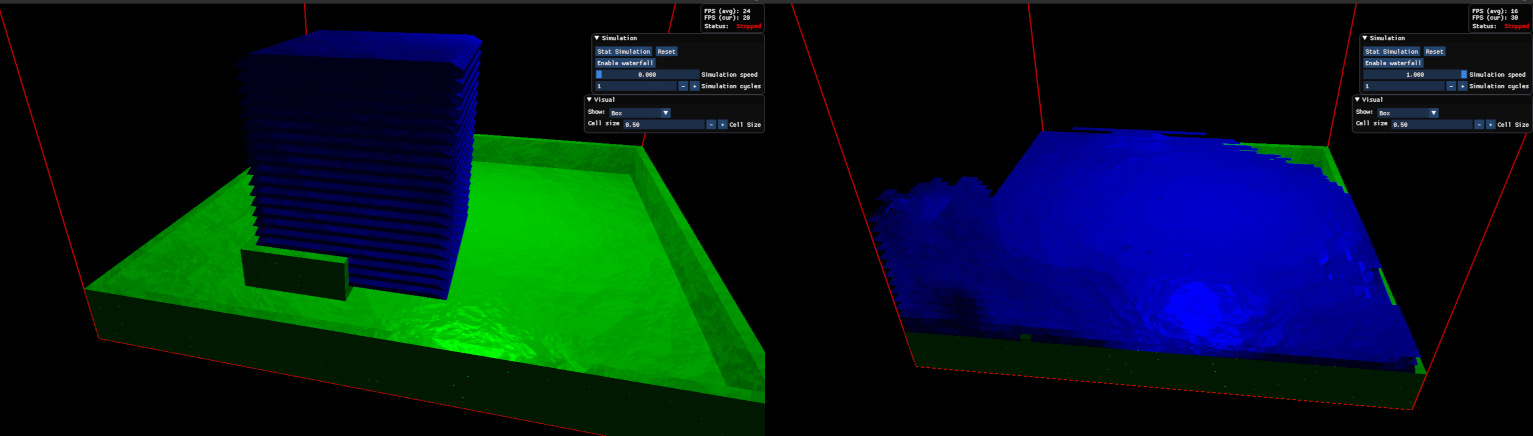
\includegraphics[scale=1]{images/velo.png}
    \caption{Chování metody -- vlevo počáteční konfigurace}
    \label{fig:velo}
\end{figure}

\subsection{Použité technologie}
Aplikace je implementována v jazyce c++20 a GLSL\footnote{\url{https://www.khronos.org/opengl/wiki/OpenGL_Shading_Language}}. Aplikace využívá knihovny geGL\footnote{\url{https://github.com/dormon/geGL}} pro binding OpenGL a pomocné třídy. Dále je zde využito knihovny sdl2cpp\footnote{\url{https://github.com/dormon/SDL2CPP}} pro snadnou práci s SDL2. Jako build systém je využit CMake\footnote{\url{https://cmake.org/}}

Další využité knihovny třetích stran jsou: \{fmt\}\footnote{\url{https://github.com/fmtlib/fmt}}, glm\footnote{\url{https://glm.g-truc.net/0.9.9/index.html}}, imgui\footnote{\url{https://github.com/ocornut/imgui}}, tinyobjloader\footnote{\url{https://github.com/syoyo/tinyobjloader}}.

Pro vývoj jsme využili IDE CLion\footnote{\url{https://www.jetbrains.com/clion/}} a služby GitHub\footnote{\url{https://www.github.com}} pro hostování zdrojových kódů.

\newpage
\section{Vykreslování}
Pro vykreslení je použito poměrně primitivní metody. Za předpokladu, že každou buňku mřížky vykreslujeme jako krychli (resp. obdelník), můžeme využít znalost zaplnění okolních buněk a tím přizpůsobit výšku hladiny vůči sousedním buňkám. Algoritmus je následující:
\begin{enumerate}
    \item Vertex shader předá geometry shaderu informace o stavu buňky a zároveň vypočítá pozice buněk pomocí MVP matic.
    \item Geometry shader zkontroluje, zda-li buňka obsahuje nějakou kapalinu. Pokud ano, pokračujeme dále.
    \item Pro každou hranu buňky kolmou k rovině Y spočítá zaplnění sousedů, zprůměruje a vytvoří tím výšku zaplnění v dané hraně.
    \item Na základě vypočtených hodnot jsou vystreamovány vertexy reprezentující vodu v buňce.
    \item Ve fragment shaderu dochází k aplikaci osvětlení na fragmenty a také jednoduchému normal mapping založeném na fraktálovém šumu.
\end{enumerate}

Výsledek vykreslování je na obrázku \ref{fig:render}.


\begin{figure}[H]
    \centering
    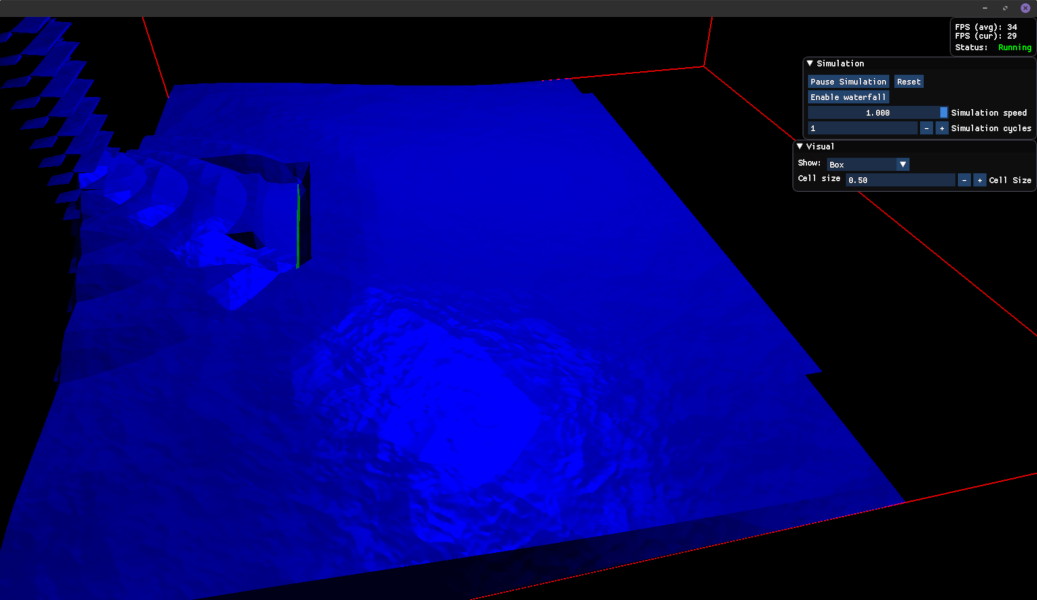
\includegraphics[scale=1.5]{images/render.png}
    \caption{Ukázka vykreslené vody}
    \label{fig:render}
\end{figure}

\section{Ovládání aplikace}
V demonstrační aplikaci je několik prvků, které umožňují změnit její chování. První částí je simulation:

\begin{figure}[H]
    \centering
    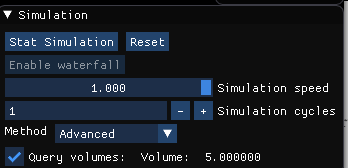
\includegraphics[scale=2]{images/sim.png}
    \caption{UI pro ovládání simulace}
    \label{fig:simui}
\end{figure}

Umožňuje zapnout/pozastavit simulaci, případně ji restartovat. Také umožňuje měnit rychlost simulace, její typ a počet cyklů simulace v jednom snímku. Zobrazuje celkové množství kapaliny v simulovaném prostoru.

Dalším prvkem je ovládání vykreslování. Umožňuje nastavit zobrazení okrajů buněk či prostoru vymezeného simulací. Také umožňuje přepnout do módu, kdy každá buňka je vykreslena barvou odpovídající jejímu zaplnění -- méně zaplněné buňky se blíží více k červené než k modré barvě, buňky zaplněné nad klidovou maximální kapacitu jsou vykresleny zeleně. Poslední modifikovatelný parametr je velikost buněk v prostoru. Také umožňuje výběr jedné z předpřipravených demonstračních map.

\begin{figure}[H]
    \centering
    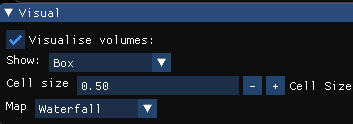
\includegraphics[scale=2.3]{images/visual.png}
    \caption{UI pro ovládání vykreslování}
    \label{fig:simui}
\end{figure}


\section{Časová a paměťová náročnost}
Vzhledem k tomu, že veškerá data použita k simulaci jsou uložena v paměti grafické karty, se budeme zaobírat pouze využitím VRAM. 

Všechna měření času byla prováděna 100 000-krát a následně zprůměrována. Měření bylo provedeno pro prázdnou mřížku, zaplněnou z 50\% a plnou. Testováno na NVidia GTX 660 Ti.

\subsection{První metoda}
Každá buňka obsahuje následující data: obsah tekutiny (float), bitové pole pro příznaky (integer), obsah tekutiny v mezikroku (float). Celkově tedy každá buňka zabírá 12 bytů VRAM paměti.Vzhledem k tomu, že potřebujeme pro výpočet 2 kopie buňky (1 ze současného kroku, druhá pro budoucí), je paměťová náročnost zdvojnásobena, tedy na každou buňku spadá 24 bytů.

\begin{figure}[H]
    \centering
    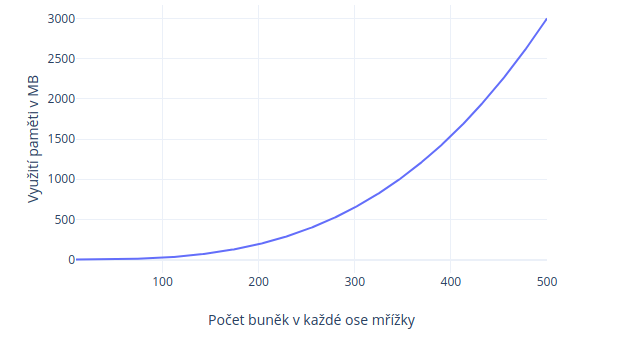
\includegraphics[scale=2]{images/memory.png}
    \caption{Závislost využité paměti na velikosti mřížky buněk}
    \label{fig:mem}
\end{figure}

Časová náročnost je samozřejmě závislá na velikosti počítané mřížky a také na momentálním stavu zaplnění. V tabulce níže najdete naměřené hodnoty společně s informacemi o velikosti a zaplnění mřížky.

\begin{table}[H]
\begin{tabular}{|l|l|l|l|l|}
\hline
Mřížka & Buňky (tisíce) & Čas - prázdný grid (\mu s) & Čas - 50\% grid (\mu s) & Čas - plný grid (\mu s) \\\hline
10                 & 1                    & 0.69                      & 0.96                           & 0.94                   \\ \hline
20                 & 8                    & 0.93                      & 1.12                           & 1.08                   \\ \hline
50                 & 125                  & 58                        & 73                             & 70                     \\ \hline
100                & 1000                 & 1014                      & 1385                           & 1257                   \\ \hline
200                & 8000                 & 3120                      & 4203                           & 3830                   \\ \hline
\end{tabular}
\end{table}

\subsection{Druhá metoda}
Pro tuto metodu potřebujeme v každé buňce informaci o obsahu kapaliny (float) a rychlosti a směru pohybu (3 float). Tyto hodnoty jsou použity 2x, podobně jako pro metodu předchozí. Dále pro mezi-výpočty používáme 2x vektor pohybu (6 float), příznaky (integer). Celková potřebná paměť pro jednu buňku je tedy 44 bytů. 
\begin{figure}[H]
    \centering
    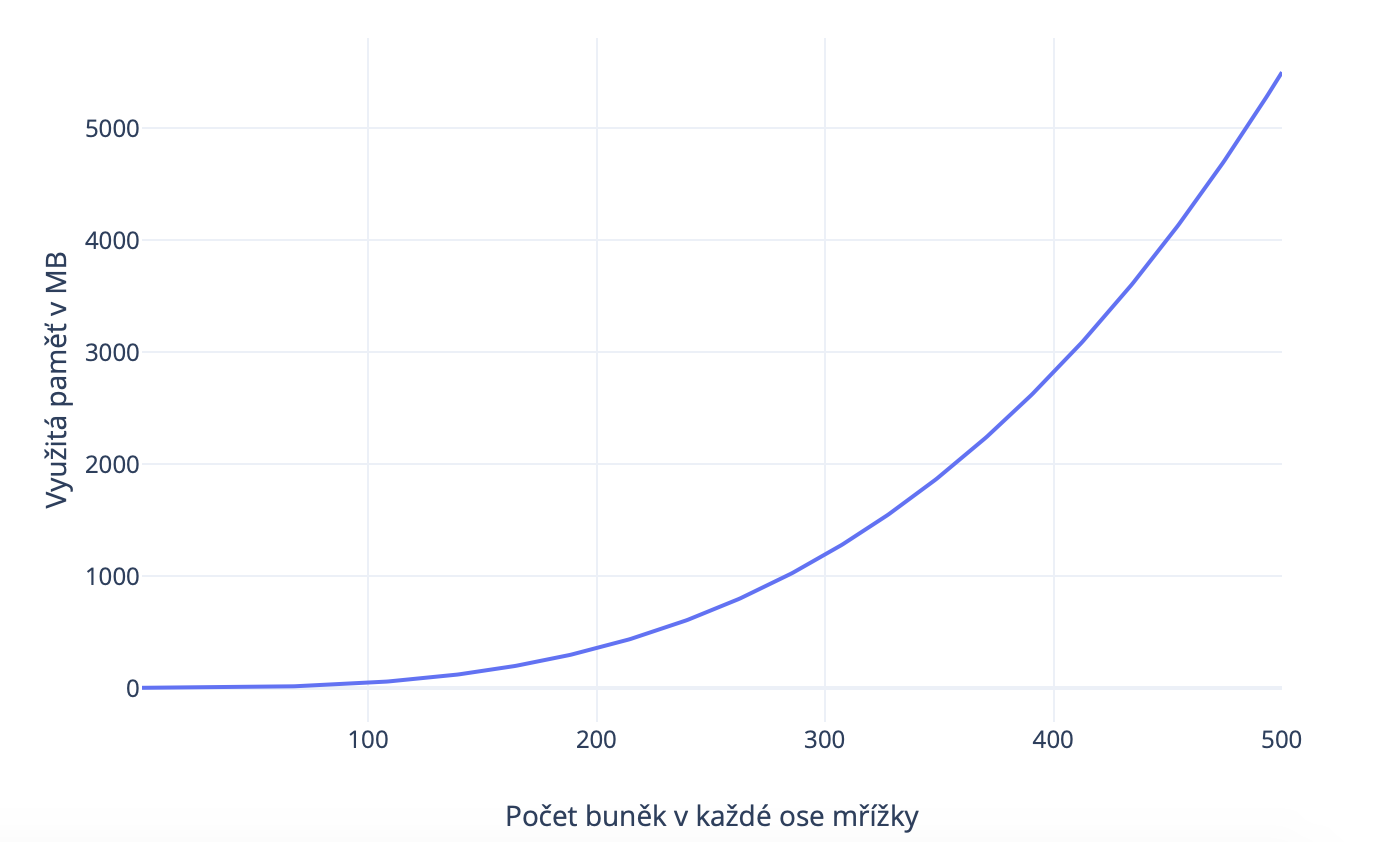
\includegraphics[scale=0.5]{images/mem2.png}
    \caption{Závislost využité paměti na velikosti mřížky buněk}
    \label{fig:mem}
\end{figure}

Časová náročnost, podobně jako v předchozím případě, je opět závislá na velikosti mřížky a stavu zaplnění. V tabulce níže jsou uvedeny hodnoty s informacemi o zaplnění mřížky. 

\begin{table}[H]
\begin{tabular}{|l|l|l|l|l|}
\hline
Mřížka & Buňky (tisíce) & Čas - prázdný grid (\mu s) & Čas - 50\% grid (\mu s) & Čas - plný grid (\mu s) \\\hline
10                 & 1                    & 15                      & 90                           & 87                   \\ \hline
20                 & 8                    & 50                      & 278                          & 282                   \\ \hline
50                 & 125                  & 343                        & 1830                             & 1943                     \\ \hline
100                & 1000                 & 2909                      & 12321                           & 13823                   \\ \hline
200                & 8000                 & 15877                      & 83231                           & 95262                   \\ \hline
\end{tabular}
\end{table}

\newpage
\section{Závěr}
V programu jsme implementovali dvě metody. U první metody jsme se soustředili především na jednoduchost a rychlost. Metoda však není dostatečně fyzikálně přesná a tekutina působí silně viskózně.

U druhé metody jsme se proto soustředili na lepší reprezentaci fyzikálních vlastností vody. V této metodě se pokoušíme simulovat především odrazy a vnitřní tlak. Metoda v určitých případech opravdu působí na oko mnohem "realističtěji", nicméně má několik nedostatků jako vyšší výpočetní náročnost, či vysoký neklid hladiny.

Celkově jsme si na tomto projektu vyzkoušeli především práci s compute shadery, paralelní myšlení a výhody a nevýhody programování na GPU. Celkově by se program dal dále rozšířit o načítání terénu ze souboru, vylepšení pokročilejší metody, případně zlepšení vizuální stránky například aplikováním Marching cubes na povrch tekutiny. 

\nocite{Medvecky_Heretik2018thesis}
\bibliographystyle{plain}
\begin{flushleft}
  \bibliography{references}
\end{flushleft}

\end{document}

